%--------------------------------------------------------------------------------------------------------------------------------------------
%General Stuff
%--------------------------------------------------------------------------------------------------------------------------------------------
\section{Simplex}
Ein Simplex ist ein Begriff, welcher aus der Geometrie stammt. Er beschreibt ein n-dimensionales Polytop. Wobei ein Polytop die Bezeichnung für ein verallgemeinertes Polygon ist, sprich ein verallgemeinertes Vieleck. 
Hier einige vorstellbare Beispiele zum Simplex:\\
 
\begin{tabular}{c|l}
Dimension & Geometrische Form\\
\hline
$n=0$ & Punkt\\
$n=1$ & Strecke\\
$n=2$ & Dreieck\\
$n=3$ & Tetraeder
\end{tabular} 

Aus der Tabelle wird ersichtlich, dass jeder n-dimensionale Simplex genau n+1 Ecken hat.

Im Downhilh-Simplex-Verfahren wird der Simplex benötigt, um die optimalen Parameterwerte zu finden. Man kann es sich so vorstellen, dass der Simplex im n-dimensionalen Parameterraum aufgespannt wird und dann für jeden Punkt des Simplex die Fehlerfunktion berechnet wird.

Der schlechteste dieser Punkte wird dann mittels gewisse "Taktiken" ersetzt und dies wird solange fort geführt, bis das Ergebnis erreicht worden ist. 

%--------------------------------------------------------------------------------------------------------------------------------------------

\section{Modifikationen des Simplex}
Die Möglichkeiten den Simplex soweit zu verändern, dass er den optimalen Punkt findet, sind begrenzt.

Es gibt einige Modifikationen, welche man auf den Simplex anwenden kann. Die Darstellungen beziehen sich hierbei auf einen Simplex der zweiten Dimension (Dreieck), natürlich gelten diese Modifikationen auch für den n-dimensionalen Simplex.

\begin{figure}[h]
	\centering
	
\usetikzlibrary{arrows}

\definecolor{uuuuuu}{rgb}{0.27,0.27,0.27}
\definecolor{zzttqq}{rgb}{0.6,0.2,0}
\definecolor{qqqqff}{rgb}{0,0,1}
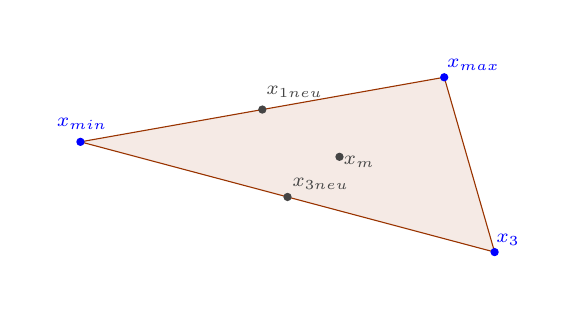
\begin{tikzpicture}[line cap=round,line join=round,>=triangle 45,x=1.0cm,y=1.0cm]
\clip(5.07,1.09) rectangle (11.72,4.37);
\fill[color=zzttqq,fill=zzttqq,fill opacity=0.1] (5.74,2.92) -- (10.36,3.74) -- (11,1.52) -- cycle;
\draw [color=zzttqq] (5.74,2.92)-- (10.36,3.74);
\draw [color=zzttqq] (10.36,3.74)-- (11,1.52);
\draw [color=zzttqq] (11,1.52)-- (5.74,2.92);
\begin{scriptsize}
\fill [color=qqqqff] (5.74,2.92) circle (1.5pt);
\draw[color=qqqqff] (5.76,3.15) node {$x_{min}$};
\fill [color=qqqqff] (10.36,3.74) circle (1.5pt);
\draw[color=qqqqff] (10.73,3.9) node {$x_{max}$};
\fill [color=qqqqff] (11,1.52) circle (1.5pt);
\draw[color=qqqqff] (11.17,1.68) node {$x_3$};
\fill [color=uuuuuu] (8.05,3.33) circle (1.5pt);
\draw[color=uuuuuu] (8.46,3.56) node {$x_{1neu}$};
\fill [color=uuuuuu] (8.37,2.22) circle (1.5pt);
\draw[color=uuuuuu] (8.79,2.39) node {$x_{3neu}$};
\fill [color=uuuuuu] (9.03,2.73) circle (1.5pt);
\draw[color=uuuuuu] (9.28,2.67) node {$x_m$};
\end{scriptsize}
\end{tikzpicture}
%
  	\caption{bla}%
	\label{fig:Dreiecke}%
\end{figure}


